\section{Design}
\label{sec:design}

In this section I go over the high level overview of my tools design. Starting with the high level, and going into more depth looking at each module.

\subsection{High level Overview}
\label{subsec:high_level_overview}

From the start I wanted to build a system, that was modular and self-contained. However, as the project went on a few adjust had to my original design. When I ran into some implementation problems discussed in the next chapter. The figure~\ref{fig:design_old} shows the original design.

\begin{figure}[H]
	\centering
	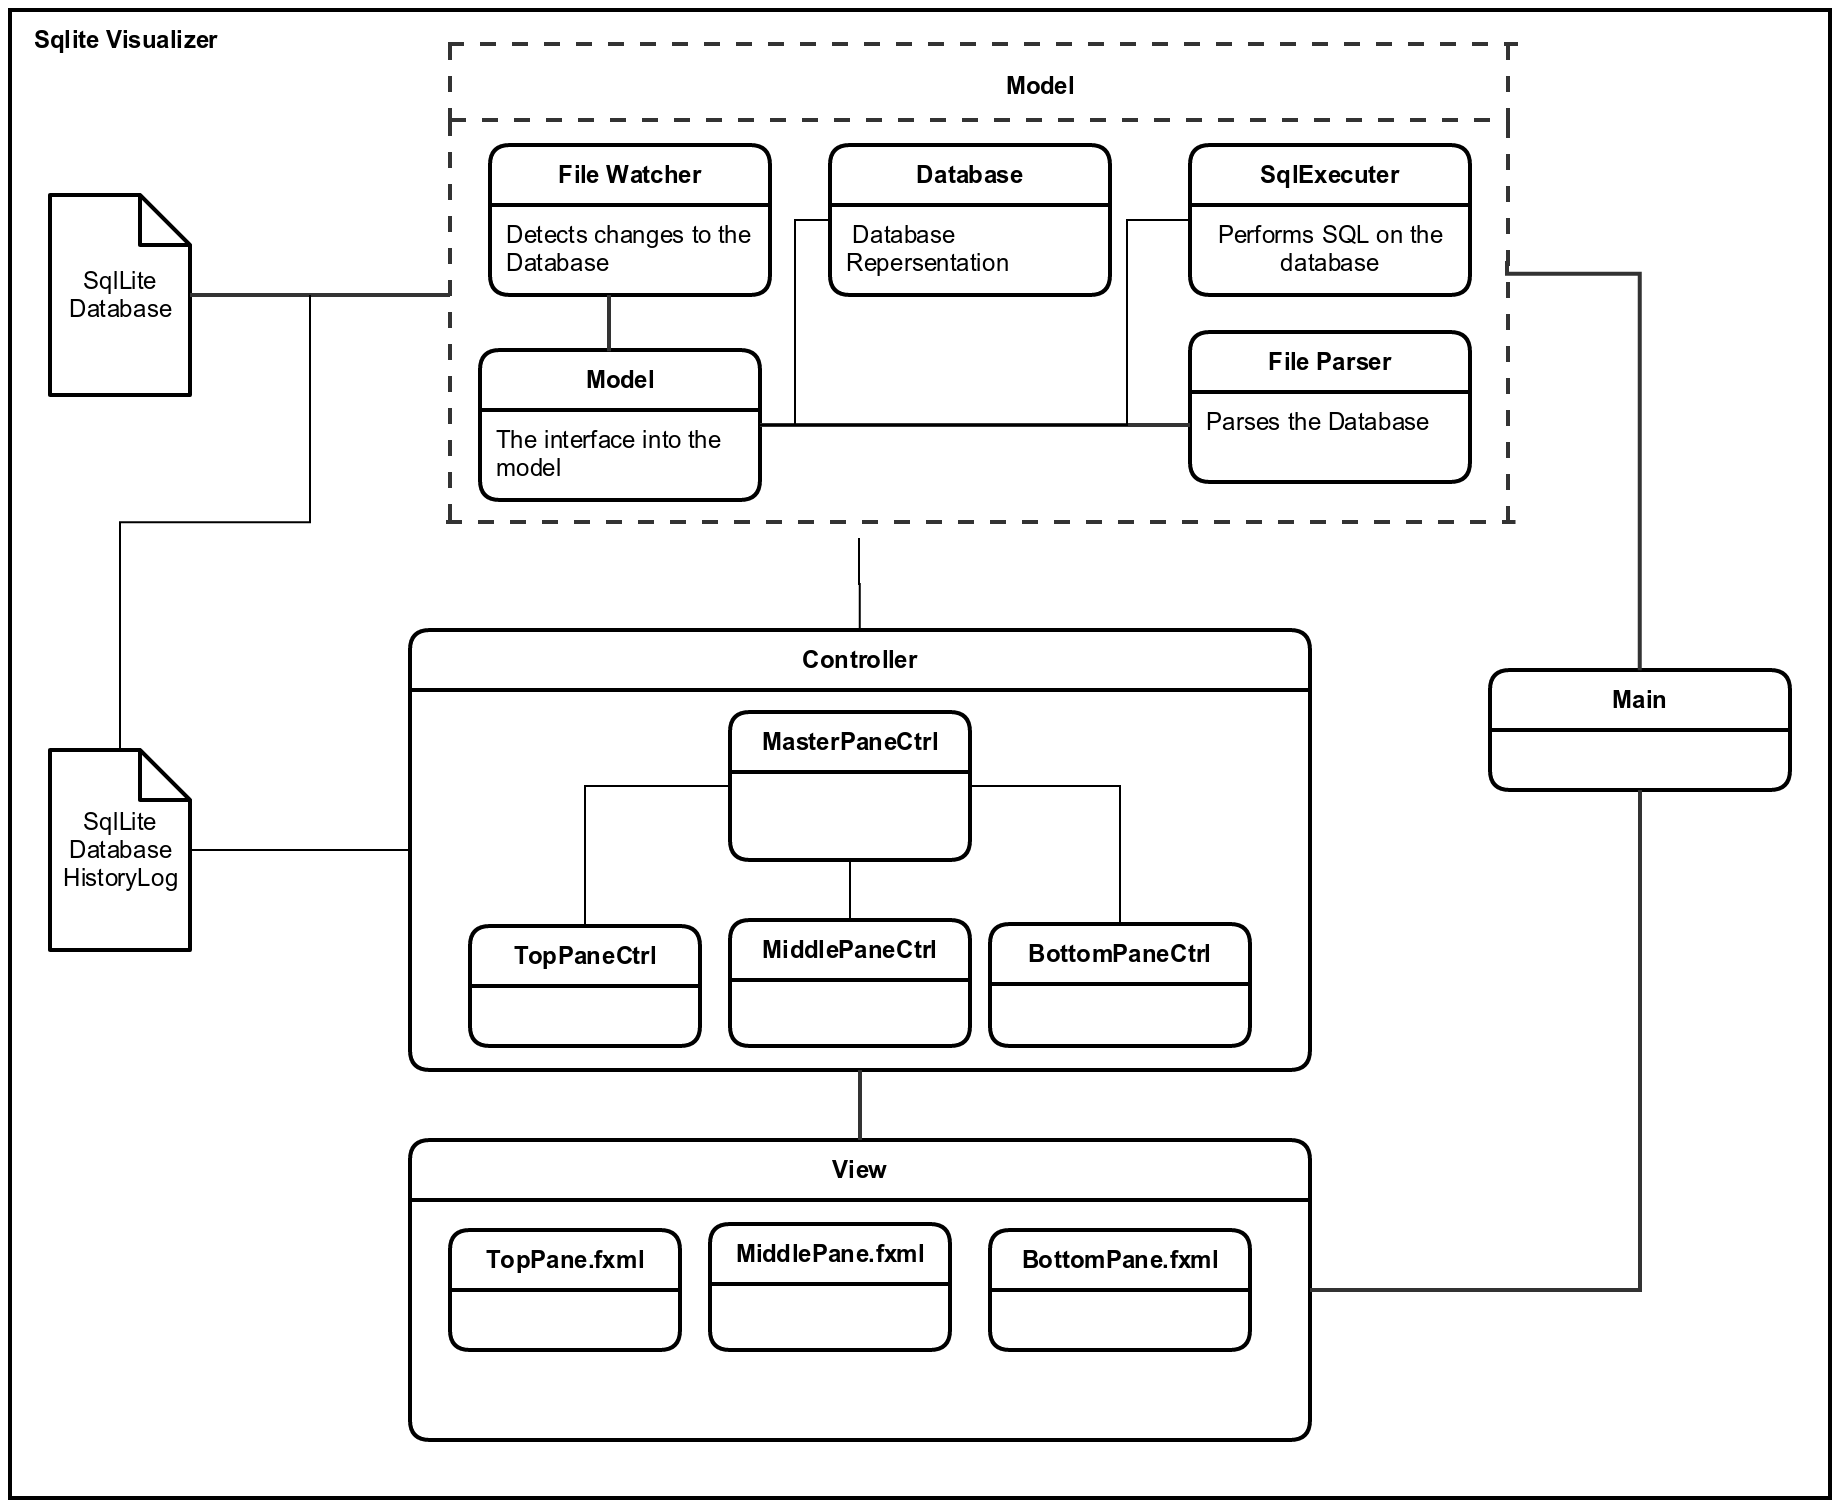
\includegraphics[scale=0.2]{images/system_diagram_old.png}
	\caption{Original system diagram}
	\label{fig:design_old}
\end{figure}

As you can see, the design utilizes the MVC (Model-View-Controller) style architect in order to separate the interface from the data. The idea being that the view could be switched out at anytime without breaking the application.
\\\\
The Model was going to run in its own thread so it could control, manage and prepare the data as it came in. This meant the view could request it when it wanted. One other thing to note, is the command logging was going to store them in to an external file, for the view. However, this design proved unusable and thus changed into the following seen in figure~\ref{fig:design_new}. 

\begin{figure}[H]
	\centering
	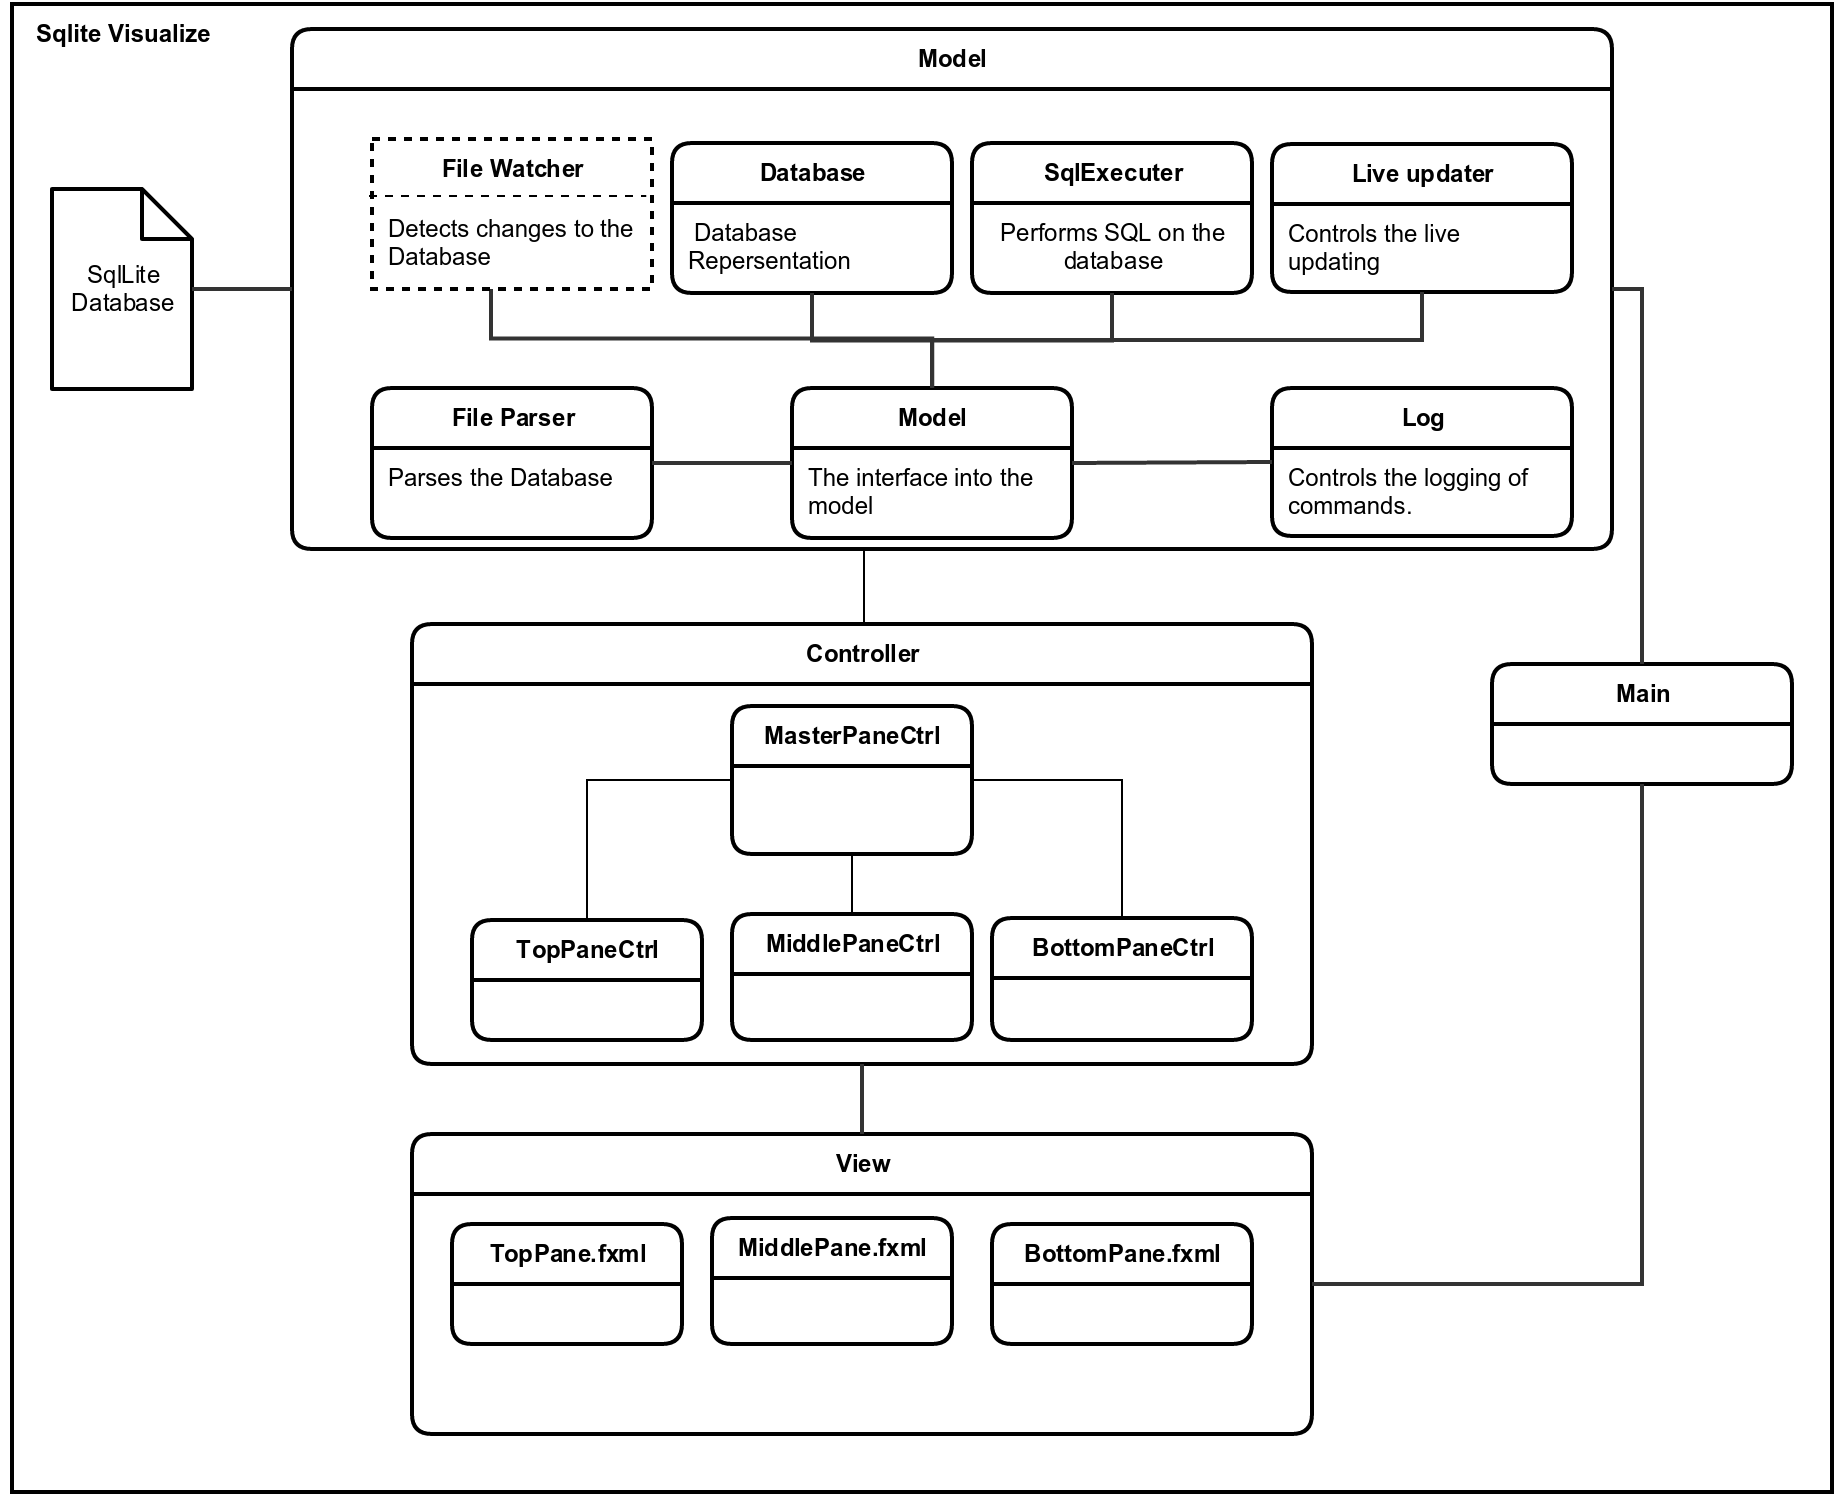
\includegraphics[scale=0.2]{images/system_diagram_new.png}
	\caption{Final system diagram}
	\label{fig:design_new}
\end{figure}

Most of the changes are seen within the Model, with the addition of two new modules. And rather then running the whole thing inside a new thread only the file watcher is. On top of this the command logging is no longer written out to file. I will go over each of the modules in the next part.

\subsection{Module Overview}
\label{subsec:module_overview}

The first module..